\documentclass[11pt]{article}
\usepackage{fontspec}
\usepackage[margin=25mm]{geometry}
\usepackage{graphicx}
\usepackage{hyperref}
\title{Skill-guided agentic finite element analysis for nonlinear static verification of bridge catwalks}
\date{}
\begin{document}
\maketitle
\noindent Reference-led manuscript outline. Compile with XeLaTeX or LuaLaTeX.
\section*{I. Introduction}
\textit{Reference anchor: I. Introduction, pp. 1–2}
\begin{enumerate}
\item Paragraph 1 — Introduce agentic engineering workflows through the sequence used in FeaGPT: language-based task specification, tool execution and computational engineering results. Cite FeaGPT at the transition to finite element analysis.
\item Paragraph 2 — Move from the reference aircraft/component setting to bridge catwalk verification. Describe the practical input chain: a prestressed INP model, six load combinations, an existing engineering report and a required reproducible calculation package.
\item Paragraph 3 — Define the central workflow problem: preserving model identity, prestress, stepwise total loads and result-group definitions across automated execution. Use the P5 file-version/load-history episode as the motivating example.
\item Paragraph 4 — Introduce the Skill as the executable analysis specification, then list the paper contributions in the reference order: structured task execution; Gmsh–CalculiX integration; six-case quantitative verification; automatic engineering-report delivery.
\end{enumerate}
\section*{II.A. System overview}
\textit{Reference anchor: II.A. System Overview, p. 3; Fig. 1}
\begin{enumerate}
\item Describe the four workflow modules and their file interfaces using Figure 1. The assistant reads the English Skill and invokes the packaged tools; each tool produces named, machine-readable evidence.
\item Identify the model asset manifest, original PDF, benchmark JSON and font/style assets. Trace one request from asset verification to the report and raw solver package.
\end{enumerate}
\section*{II.B. Skill-guided planning and task orchestration}
\textit{Reference anchor: II.B. Engineering Analysis Planning and Task Orchestration, pp. 3–6; Algorithm 1}
\begin{enumerate}
\item Replace the reference geometry-design JSON with the catwalk task schema: input manifest, cases P1–P6, solver identity, units, execution stages, comparison criteria and report outputs.
\item Present Algorithm 1 as the executable order: validate → reconstruct mesh → solve each case → read final fields → recover forces → compare → generate report → hash outputs. State the stage-specific completion conditions.
\item For the planned GLM execution experiment, record provider/model identifier, request, tool calls, elapsed time, retries and final artifact status in a session log. Fill the model identifier from the actual run.
\end{enumerate}
\section*{II.C. Versioned model reconstruction and engineering knowledge}
\textit{Reference anchor: II.C. Intelligent Geometry Generation with Knowledge Augmentation, pp. 6–7; Fig. 2}
\begin{enumerate}
\item Describe reconstruction from the original coordinates and connectivity, followed by material/section/support audit. Use Figure 2 to connect global geometry, structural families and a local connection.
\item Give the equivalent material values from the INP: MAT1/MAT2 E = 120 GPa, areas 22298.692/8402.9797 mm² and their equivalent densities; MAT3 E = 206 GPa, rectangular section 98.954535 × 98.954535 mm and near-zero assigned density.
\item Describe 8,984 initial-stress records across 1,123 cable elements, the global tensor convention and the retained reference geometry. Link numerical values to the material table and asset hashes.
\end{enumerate}
\section*{II.D. Gmsh mesh generation and identity mapping}
\textit{Reference anchor: II.D. Adaptive Mesh Generation, pp. 7–8; Fig. 3; Table II}
\begin{enumerate}
\item Explain point/line creation from INP IDs, section physical groups, setTransfiniteCurve(eid, 2), first-order generate(1), and MSH 4.1 export.
\item Distinguish geometric tags from mesh tags. Describe the explicit node/element mapping and checks: node count, element count, coordinates and ordered endpoints. Table II reports the measured mesh identity results.
\end{enumerate}
\section*{II.E. Nonlinear static analysis and load-history execution}
\textit{Reference anchor: II.E. Automated FEA Simulation and Analysis, pp. 8–9}
\begin{enumerate}
\item Write equilibrium as R(u, λ) = fint(u, σ0, T) − fext(λ) = 0. Describe geometric nonlinearity, initial prestress, gravity and prescribed supports within the planar X–Z system.
\item State the six combinations in Table I. P1 contains one dead-load step; P2–P6 independently establish dead load before their target total combination. Explain the second-step CLOAD total convention, with P5 as the worked example.
\item Give g = 9806 mm/s², alpha = 1.2e-5 /°C for P3/P6, temperature changes −15/−34°C and the 1,125 UY constraints. Identify the locked solver build and final-time checks.
\end{enumerate}
\section*{II.F. Field recovery and automated verification}
\textit{Reference anchor: II.F. Intelligent Data Analysis and Batch Processing, p. 9}
\begin{enumerate}
\item Define Umax = max sqrt(UX²+UY²+UZ²) over original nodes. Define the deformed chord n and recover N = A0 nᵀ σbar n / 1000 in kN, averaging the eight integration-point tensors.
\item Define eight reporting span groups, their maxima and K = Nbreak/Nmax. Set Nbreak = 38080/14280 kN and give the case-specific K requirements.
\item Define signed relative difference δ = 100(qcalc/qref − 1). Identify the independent MAPDL displacement source and the report force tables separately. Describe Figure 4 and the machine-readable evidence files.
\end{enumerate}
\section*{II.G. Reproducible batch execution and report generation}
\textit{Reference anchor: II.G. Scalable Batch Processing Architecture, pp. 9–10}
\begin{enumerate}
\item Describe independent case directories, common geometry audit, recorded solver commands, failure preservation and per-stage status.
\item Trace one final response value into CSV, VTU, PNG and the engineering report. Describe the shared result model used for Word/PDF and the style/font assets reproducing the reference report.
\item State the deliverable structure: six solved cases, 42 field plots, comparison data, Gmsh mapping, hashes and a 17-page engineering report in both formats.
\end{enumerate}
\section*{III.A. Task specification and six-case execution}
\textit{Reference anchor: III.A. Natural Language Input and System Understanding, p. 11; Table I}
\begin{enumerate}
\item Present the task request and its mapped case/output specification. Table I enumerates the six combinations and required safety factors.
\item For the GLM session, insert the recorded model ID and stage-completion log. Report execution and retry counts from that log.
\end{enumerate}
\section*{III.B. Model reconstruction results}
\textit{Reference anchor: III.B. Geometry Generation Results, pp. 11–12; Fig. 2}
\begin{enumerate}
\item Report 1,125 original nodes, 1,123 T3D2 cable elements and 71 B31 equivalent members. Show the complete geometry and member assignments in Figure 2.
\item Report the common geometric/physical definitions across cases and the preserved initial-stress record count.
\end{enumerate}
\section*{III.C. Mesh identity and mapping results}
\textit{Reference anchor: III.C. Mesh Generation and Quality Analysis, pp. 12–13; Table II; Fig. 3}
\begin{enumerate}
\item Report identical node/element counts, zero coordinate discrepancy and matching ordered connectivity between the input and the Gmsh mesh. Use the local inset to display the mapping.
\item Explain how this identity connects solved fields to the displayed geometry and reporting groups.
\end{enumerate}
\section*{III.D. Nonlinear response and benchmark comparison}
\textit{Reference anchor: III.D. FEA Simulation and Results Analysis, p. 14; Table III}
\begin{enumerate}
\item Report completion of all six cases and matching peak-displacement node IDs. Present the six numerical rows in Table III.
\item Give maximum absolute differences: displacement 0.859887\%, bottom-cable span force 0.853551\% and portal-cable span force 1.125518\%. Identify the controlling case/span from the supplied evidence table.
\item Discuss P4 as the largest peak-displacement response, P5 peak at node 306, and the P3/P6 cooling responses using the solved fields.
\end{enumerate}
\section*{III.E. Cable response interpretation and safety assessment}
\textit{Reference anchor: III.E. Intelligent Result Analysis and Autonomous Design Evaluation, pp. 14–16; Fig. 4}
\begin{enumerate}
\item Follow the four panels in order: global displacement agreement, span-force agreement, cable safety factors and the spatial/case distribution of signed differences.
\item Compare the governing bottom/portal factors by case with Table I requirements. Use the heatmap to locate differences while retaining cable family and span identity.
\item Explain the load-history correction through the P5 input audit: second-step total nodal load includes the first-step permanent contribution. Connect the input definition with the current node-306 downward response.
\end{enumerate}
\section*{III.F. Execution performance and automation accounting}
\textit{Reference anchor: III.F. Computational Performance and Scalability, pp. 16–17}
\begin{enumerate}
\item Report the recorded solver wall times by case and their sum, with Python/platform/solver identity. Label timing boundaries explicitly.
\item Add the planned GLM session measurements in a separate table: planning time, tool time, report-generation time, total session time, token usage when exposed by the provider, retries and completion count.
\item For repeated-session evaluation, use the same six inputs and output contract; record each session independently before calculating completion rate and timing distributions.
\end{enumerate}
\section*{III.G. Engineering case presentation and report delivery}
\textit{Reference anchor: III.G. Industrial Validation: CalculiX Configuration Generation, pp. 17–18; Fig. 5}
\begin{enumerate}
\item Present Figure 5 as the engineering field plate: three representative cases and two response quantities. Compare shared field scales within each row.
\item Show how the prescribed report style is generated from the same result set, and point to the supplementary six-case contour plates, Word/PDF report and raw result archive.
\end{enumerate}
\section*{IV. Conclusions}
\textit{Reference anchor: IV. Conclusions, pp. 18–19}
\begin{enumerate}
\item Conclusion 1 — Summarize the Skill-guided sequence connecting versioned bridge inputs to mesh verification, nonlinear solution and engineering-report generation.
\item Conclusion 2 — State the measured mesh identity and six-case response differences with their actual values.
\item Conclusion 3 — State the cable safety-factor outcomes and delivered evidence package. Add session-level GLM findings after inserting the measured session table.
\end{enumerate}
\begin{figure}[ht]
\centering
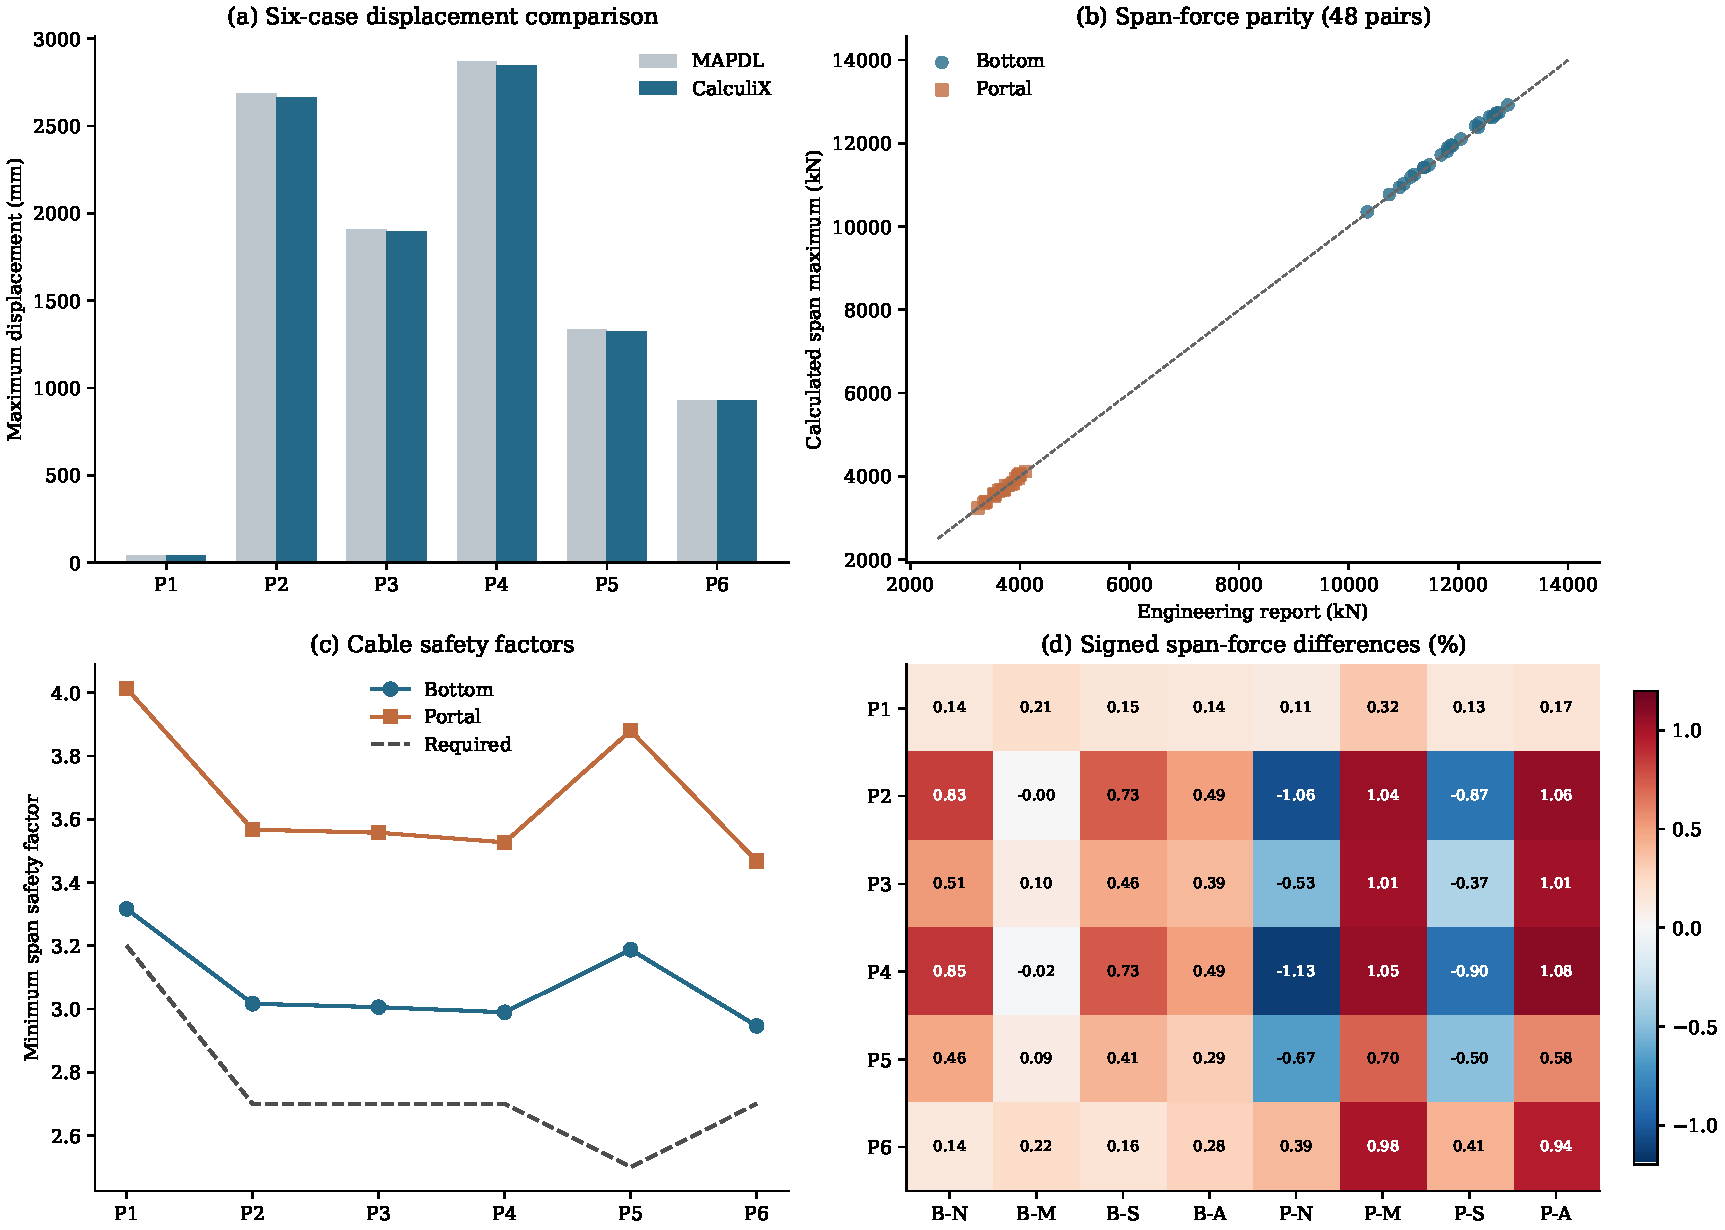
\includegraphics[width=\textwidth]{figures/figure_4_six_case_verification.pdf}
\caption{Figure 4. Six-case verification: (a) maximum displacement compared with MAPDL; (b) 48 span-force comparisons with the engineering report; (c) minimum span safety factors and required values; (d) signed force differences by case and span.}
\end{figure}
\begin{thebibliography}{9}
\bibitem{qi2025feagpt} Qi, Y., Xu, R., and Chu, X. FeaGPT: an End-to-End agentic-AI for Finite Element Analysis. arXiv:2510.21993v1 (2025). https://arxiv.org/abs/2510.21993v1
\end{thebibliography}
\end{document}
